\documentclass{article}
% For math environments
\usepackage{amsmath, amsfonts}
% For links
\usepackage[colorlinks=true,
    linkcolor = blue,
    urlcolor  = blue,
    citecolor = blue,
    anchorcolor = blue]{hyperref}
% Put space between paragraphs
\usepackage{parskip}
% For figures
\usepackage{tikz}
% Set the margins to not be ridiculous
\usepackage[margin=0.75in]{geometry}
% For multiple columns
\usepackage{multicol}
% For controlling enum/itemize spacing and indentation
\usepackage{enumitem}
% More math symbols
\usepackage{amssymb}
% To change enumerate labels

% For tikz plots
\usepackage{pgfplots}
% This isn't needed but avoids a compiler warning
\pgfplotsset{compat=1.16}

% Allow multi-line equations to be broken across pages
\allowdisplaybreaks

% Use @ as a letter
\makeatletter

% Scale down all tikz coordinates while maintaining font size
\tikzset{every picture/.style={scale=0.45, every picture/.style={}}}


% Macros
% Monospace code
\def\code#1{\texttt{#1}}

% Greek letters
\def\a{\alpha}
\def\b{\beta}
\def\g{\gamma}
\def\d{\delta}
\def\D{\Delta}

% Commands that make life easier
\newcommand\gath[1]{\begin{gather} #1 \end{gather}}
\newcommand\ali[1]{\begin{align} #1 \end{align}}
\newcommand\parens[1]{\left( #1 \right)}
\newcommand\squares[1]{\left[ #1 \right]}
\newcommand\braces[1]{\left\{ #1 \right\}}
\newcommand\angles[1]{\left\langle #1 \right\rangle}
\newcommand\deriv[2]{\frac{d #1}{d #2}}
\newcommand\abs[1]{\left| #1 \right|}
\newcommand\floor[1]{\left\lfloor #1 \right\rfloor}
\DeclareMathOperator{\lcm}{lcm}
\def\non{\nonumber \\}

% Multiline equation space
\def\mlesp{\hspace{1.2cm}}

% For grid diagrams
\newcommand\gridbox[3]{\draw (#1,#2) rectangle (#1+1,#2+1) node[pos=.5] {#3};}
\newcommand\gridboxh[3]{\draw[fill=red!20] (#1,#2) rectangle (#1+1,#2+1) node[pos=.5] {#3};}
\newcommand\gridboxb[3]{\draw[fill=black] (#1,#2) rectangle (#1+1,#2+1) node[pos=.5] {#3};}
\newcommand\gridsym[3]{\node at (#1+0.5,#2+0.5) {$#3$};}
\newcommand\gridblank[2]{\filldraw[draw=gray, color=gray] (#1,#2) rectangle (#1+1,#2+1);}
\newcommand\gridcirc[2]{\draw (#1 + 0.5,#2 + 0.5) circle (0.25);}
\newcommand\cwlab[3]{
  \def\dd{0.15}
  \draw (#1 + \dd - 0.03, #2 + 1 - \dd) node {\scriptsize #3};
}

\def\bbw{3.5}
\def\bbh{2}
\newcommand\bigbox[3]{\draw (#1*\bbw,#2*\bbh) rectangle (#1*\bbw+\bbw,#2*\bbh+\bbh) node[pos=.5] {#3};}
\newcommand\bbtextr[3]{\node[right] at (#1*\bbw,#2*\bbh+0.5*\bbh) {#3};}
\newcommand\bbtextb[3]{\node[align=center] at (#1*\bbw+0.5*\bbw,#2*\bbh+0.5*\bbh) {#3};}

% Box puzzle stock answer
\newcommand\boxans[1]{
  Logic was used to deduce the solution:

  #1

  This was verified using Python as well as shown to be unique with a brute force approach.
}

% Multiple numbers
\newcommand\mn[1]{$#1$'s}

% Commands for problems
\newcommand\problem[4]{
  \section*{#1}

  Question: #3
  
  Answer: #2
  
  Explanation: #4
}
\newcommand\aproblem[4]{\problem{Dec #1}{#2}{#3}{#4}}
\newcommand\cproblem[4]{\problem{Problem #1}{#2}{#3}{#4}}

\def\advent@xxiv@i{
  Eve writes down five different positive integers.
  The sum of her integers is $16$. What is the product of her integers?
}

\def\advent@xxiv@ii{
  $14$ is the smallest even number that cannot be obtained by rolling two $6$-sided dice and finding the product of the numbers rolled.

  What is the smallest even number that cannot be obtained by rolling one hundred $100$-sided dice and finding the product of the numbers rolled?
}

\def\advent@xxiv@iii{
  There are $5$ ways to write $5$ as the sum of positive odd numbers:
  \begin{itemize}
    \item $1 + 1 + 1 + 1 + 1$
    \item $1 + 1 + 3$
    \item $3 + 1 + 1$
    \item $1 + 3 + 1$
    \item $5$
  \end{itemize}

  How many ways are there to write $14$ as the sum of positive odd numbers?
}

\def\advent@xxiv@iv{
  The geometric mean of a set of $n$ numbers is computed by mulitplying all the numbers together, then taking the $n$th root.
  The factors of $9$ are $1$, $3$, and $9$.
  The geometric mean of these factors is
  \gath{
    \sqrt[3]{1 \times 3 \times 9} = \sqrt[3]{27} = 3
  }
  What is the smallest number where the geometric mean of its factors is $13$?
}

\def\advent@xxiv@v{
  The sum of $11$ consecutive integers is $2024$.
  What is the smallest of the $11$ integers?
}

\def\advent@xxiv@vi{Put the digits 1 to 9 (using each digit exactly once) in the boxes so that the sums are correct. The sums should be read left to right and top to bottom ignoring the usual order of operations. For example, 4+3×2 is 14, not 10. Today's number is the product of the numbers in the red boxes.
  The number $n$ has $55$ digits.
  All of its digits are $9$.
  What is the sum of the digits of $n^3$?
}

\def\advent@xxiv@vii{
  What is the obtuse angle in degrees between the minute and hour hands of a clock at 08:22?
}

\def\advent@xxiv@viii{
  It is possible to arrange $4$ points on a plane and draw non-intersecting lines between them to form $3$ non-overlapping triangles:

  \begin{center}
    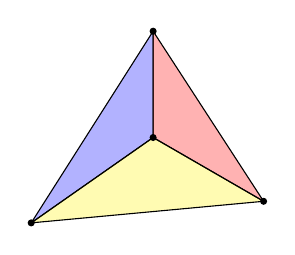
\begin{tikzpicture}
      \def\ds{3}
      \def\pa{(0: 0)}
      \def\pb{(90: \ds)}
      \def\pc{(215: 1.4*\ds)}
      \def\pd{(-30: 1.2*\ds)}

      \def\bcr{3}
      \def\scr{0.55*\bcr}
      \def\sca{34}
      \def\mcr{0.7*\bcr}
      \def\mca{142}
      \def\pr{0.1}

      % Triangles
      \draw[fill=blue,fill opacity=0.3] \pa -- \pb -- \pc -- cycle;
      \draw[fill=red,fill opacity=0.3] \pa -- \pb -- \pd -- cycle;
      \draw[fill=yellow,fill opacity=0.3] \pa -- \pd -- \pc -- cycle;

      % Points
      \fill \pa circle (\pr);
      \fill \pb circle (\pr);
      \fill \pc circle (\pr);
      \fill \pd circle (\pr);
    \end{tikzpicture}
  \end{center}

  It is not possible to make more than $3$ triangles with $4$ points.

  What is the maximum number of non-overlapping triangles that can be made by arranging $290$ points on a plane and drawing non-intersecting lines between them?
}

\def\advent@xxiv@ix{
  Put the digits $1$ to $9$ (using each digit exactly once) in the boxes so that the sums are correct.
  The sums should be read left to right and top to bottom ignoring the usual order of operations.
  For example, $4 + 3 \times 2$ is $14$, not $10$.
  Today's number is the product of the numbers in the red boxes.

  \grid@advent@xxiv@ix{}{}{}{}{}{}{}{}{}
}

\def\advent@xxiv@x{
  A number is a palindrome if it's the same when its digits are written in reverse order.

  What is the sum of all the numbers between $10$ and $100$ that are palindromes?
}

\def\advent@xxiv@xi{
  There are $6$ sets of integers between $1$ and $5$ (inclusive) that contain an odd number of numbers whose median value is $3$:

  \begin{itemize}
    \item $\braces{3}$
    \item $\braces{1,3,4}$
    \item $\braces{2,3,4}$
    \item $\braces{1,3,5}$
    \item $\braces{2,3,5}$
    \item $\braces{1,2,3,4,5}$
  \end{itemize}

  How many sets of integers between $1$ and $11$ (inclusive) are there that contain an odd number of numbers whose median value is $5$?
}

\def\advent@xxiv@xii{
  Holly picks a three-digit number.
  She then makes a two-digit number by removing one of the digits.
  The sum of her two numbers is $309$.
  What was Holly's original three-digit number?
}

\def\advent@xxiv@xiii{
  Today's number is given in this crossnumber.
  No number in the completed grid starts with $0$.

  \begin{multicols}{2}
    \crossnumstd{}{}{}{}{}{}{}{}{}

    \vfill\null
    \columnbreak

    \begin{center}
      \textbf{Across}

      \begin{tabular}{clc}
        \textbf{1} & Today's number.  & (\textbf{3}) \\
        \textbf{4} & Two times 5A.    & (\textbf{3}) \\
        \textbf{5} & A multiple of 1. & (\textbf{3})
      \end{tabular}

      \textbf{Down}

      \begin{tabular}{clc}
        \textbf{1} & Sum of digits is 15. & (\textbf{3}) \\
        \textbf{2} & Sum of digits is 19. & (\textbf{3}) \\
        \textbf{3} & Three times 5A.      & (\textbf{3})
      \end{tabular}
    \end{center}
  \end{multicols}
}

\def\advent@xxiv@xiv{
  $15^3$ is $3375$.
  The last $3$ digits of $15^3$ are $375$.

  What are the last $3$ digits of $15^{1234567890}$?
}

\def\advent@xxiv@xv{
  The number $2268$ is equal to the product of a square number (whose last digit is not $0$) and the same square number with its digits reversed: $36 \times 63$.

  What is the smallest three-digit number that is equal to the product of a square number (whose last digit is not $0$) and the same square number with its digits reversed?
}

\def\advent@xxiv@xvi{
  Put the digits $1$ to $9$ (using each digit exactly once) in the boxes so that the sums are correct.
  The sums should be read left to right and top to bottom ignoring the usual order of operations.
  For example, $4 + 3 \times 2$ is $14$, not $10$.
  Today's number is the product of the numbers in the red boxes.

  \grid@advent@xxiv@xvi{}{}{}{}{}{}{}{}{}
}

\def\advent@xxiv@xvii{
  The number $40$ has $8$ factors: $1$, $2$, $4$, $5$, $8$, $10$, $20$, and $40$.

  How many factors does the number $2^{26} \times 5 \times 7^5 \times 11^2$ have?
}

\def\advent@xxiv@xviii{
  TODO
}

\def\card@xxiv@i{
  What is the largest number you can make by using the digits $1$ to $4$ to make two $2$-digit numbers, then mutiplying the two numbers together?
}

\def\card@xxiv@ii{
  What is the largest number you can make by using the digits $0$ to $9$ to make a $2$-digit number and an $8$-digit number, then mutiplying the two numbers together?
}

\def\card@xxiv@iii{
  The expansion of $(2x+3)^2$ is $4x^2 + 12x + 9$.
  The sum of the coefficients of $4x^2 + 12x + 9$ is $25$.
  What is the sum of the coefficients of the expansion of $(30x + 5)^2$?
}

\def\card@xxiv@iv{
  What is the sum of the coefficients of the expansion of $(2x+1)^{11}$?
}

\def\card@xxiv@v{
  What is the geometric mean of all the factors of $41306329$?
}

\def\card@xxiv@vi{
  What is the largest number for which the geometric mean of all its factors is $92$?
}

\def\card@xxiv@vii{
  What is the sum of all the factors of $7^4$?
}

\def\card@xxiv@viii{
  How many numbers between $1$ and $28988500000$ have an odd number of factors?
}

\def\card@xxiv@ix{
  Eve found the total of the $365$ consecutive integers starting at $500$ and the total of the next $365$ consecutive integers, then subtracted the smaller total from the larger total.
  What was her result?
}

\def\card@xxiv@x{
  Eve found the total of the $n$ consecutive integers starting at a number and the total of the next $n$ consecutive integers, then subtracted the smaller total from the larger total.
  Her result was $22344529$.
  What is the largest possible value of $n$ that she could have used?
}


\begin{document}

\title{MS Scroggs 2019 Christmas Card Solutions}
\author{Dan Whitman}
\date{}

\maketitle

Link to the online card: \href{http://mscroggs.co.uk/blog/70}{http://mscroggs.co.uk/blog/70}

\cproblem{1}{4001}{\card@xix@i}{
  Each of the four digits of a four-digit number will be one 1000 times since there are 1000 combinations of the other three digits.
  Thus the total number of ones written in the numbers 1 to 9999 are
  $$
    4 \cdot 1000 = 4000 \,.
  $$
  Then of course 10000 only has one 1 so that the final answer is $4000 + 1 = 4001$.

  This answer was verified using Python.
}

\cproblem{2}{1849}{\card@xix@ii}{
  We have that $2N+1 = 85$ for $N = 42$ so that the answer is clearly
  $$
    \sum_{k=0}^{42} (2k+1) = 2 \sum_{k=0}^{42} k + \sum_{k=0}^{42} 1 = 2 \frac{42 \cdot 43}{2} + 43 = 43 \cdot 42 + 43 = 43 (42 + 1) = 43^2 = 1849 \,.
  $$
  This answer was verified with Python.
}

\cproblem{3}{2002}{\card@xix@iii}{
  The number $4008004$ may seem like a very random choice for an upper bound of this problem, but it is not at all.
  The key insight is that for any number $n$ a factor $k$ of $n$ must always result in two factors, namely $k$ and $n/k$, noting that this is also the case for $k=1$.
  So it seems that the number of factors of $n$ must always be even.
  However, the only exception to this occurs when $n$ is a perfect square, in which case one integer factor $k = \sqrt{n}$ generates only one distinct factor instead of two.
  Therefore only the set of integers with an odd number of factors is exactly the set of perfect squares!

  Moreover if we are interested in the number of integers between $1$ and $N^2$ (inclusive) with an odd number of factors, then this is the number of perfect squares between $1$ and $N^2$.
  Of course this will simply be the set $\{k^2 \mid 1 \leq k \leq N\}$, which of course has $N$ elements.
  We then notice that $N^2 = 4008004$ is a perfect square so that the number we seek is $N = \sqrt{4008004} = 2002$.

  This result was verified using Python using a quasi-brute force approach.
}

\cproblem{4}{130405}{\card@xix@iv}{
  Here we can leverage the results of the 2016, Dec 15 problem.
  In our case, the number of pages is
  \gath{
    P = 130404 \equiv 0 \pmod{4}
  }
  so that we do in fact have a center spread, the sum of the two center spread page numbers being
  \gath{
    s = P + 1 = 130405.
  }
}

\cproblem{5}{120306}{\card@xix@v}{
  For any circle with radius $r$, the largest quadrilateral that fits in the circle is a square whose diagonal is the diameter $d = 2r$ of the circle.
  If such a square has side length $s$ then the diagonal of the square is then
  \begin{gather*}
    \sqrt{2}s = d = 2r \\
    s = \frac{2r}{\sqrt{2}} = \sqrt{2}r
  \end{gather*}
  so that the area of the square is $A = s^2 = (\sqrt{2}r)^2 = 2r^2$.
  Now, in our case, the area of the circle is $\pi r^2 = 60153 \pi$ so that clearly $r^2 = 60153$.
  Hence the area of the square that we seek is $A = 2r^2 = 120306$.
}

\cproblem{6}{514229}{\card@xix@vi}{
  Let $f(n)$ be the number of ways to write $n$ as the sum of \mn{1} and \mn{2}.
  When you write as the sum of \mn{1} and \mn{2}, the sum must end in either $1$ or $2$: if it ends in $1$, then there are $f(n-1)$ ways to write the rest before this $1$ as the sum of \mn{1} and \mn{2}; if it ends in $2$, there are $f(n-2)$ ways to write the rest.
  This means that $f(n) = f(n-1) + f(n-2)$, or in other words the Fibonacci numbers.
  We clearly have that $f(1) = 1$, and also $f(2) = 2$ (since $2$ can only be written as $1+1$ or simply $2$).
  Python was used to calculate these recursively using these base conditions so that our answer is $f(28) = 514229$.
}

\cproblem{7}{171175}{\card@xix@vii}{
  This was calculated in Python using the NumPy function.
}

\cproblem{8}{59}{\card@xix@viii}{
  The number of zeros at the end of a number is the same as the number of \mn{10} in the product that makes the number.
  Each of these \mn{10} is made by multiplying a $5$ and a $2$.
  There will clearly be many more even numbers than multiples of $5$ in any large number, and so plenty of \mn{2} to pair with each $5$.
  Hence the number of \mn{5} will tell us how many zeros the number ends in.
  In $245!$ there will be $49$ multiples of $5$ (since $245 /5 = 49$), $9$ multiples of $5^2 = 25$ (since $\floor{245/25} = 9$), and $1$ multiple of $5^3 = 125$.
  Therefore the number of zeros at the end of $245!$ is $49 + 9 + 1 = 59$.
  This was verified using Python, which is easy because integers can be arbitrarily large.
}

\cproblem{9}{304434}{\card@xix@ix}{
  The ones digit of the sum is 7, which tells us that the ones digit has to be the one that was removed so that they are different in each number.
  If this were not the case, then the ones digit of the sum would have to be even.
  Hence our two numbers have digits $N_1 = d_5 d_4 d_3 d_2 d_1 d_0$ and $N_2 = d_5 d_4 d_3 d_2 d_1$.
  Thus the sum of $d_5$ and any carried numbers from the previous additions is $3$.
  If we assume that no digits are carried over then it follows that $N_1 = 304434$ and $n_2 = 30443$, which work!

  Python was used to verify that this is the unique answer.
}

\end{document}
